\documentclass[border=10pt]{standalone}

\usepackage{tikz}
\usepackage{tikzsymbols}
\usetikzlibrary{calc,patterns,shapes.geometric}

\def\centerarc[#1](#2)(#3:#4:#5){\draw[#1] ($(#2)+({#5*cos(#3)},{#5*sin(#3)})$) arc (#3:#4:#5);}

\begin{document}
	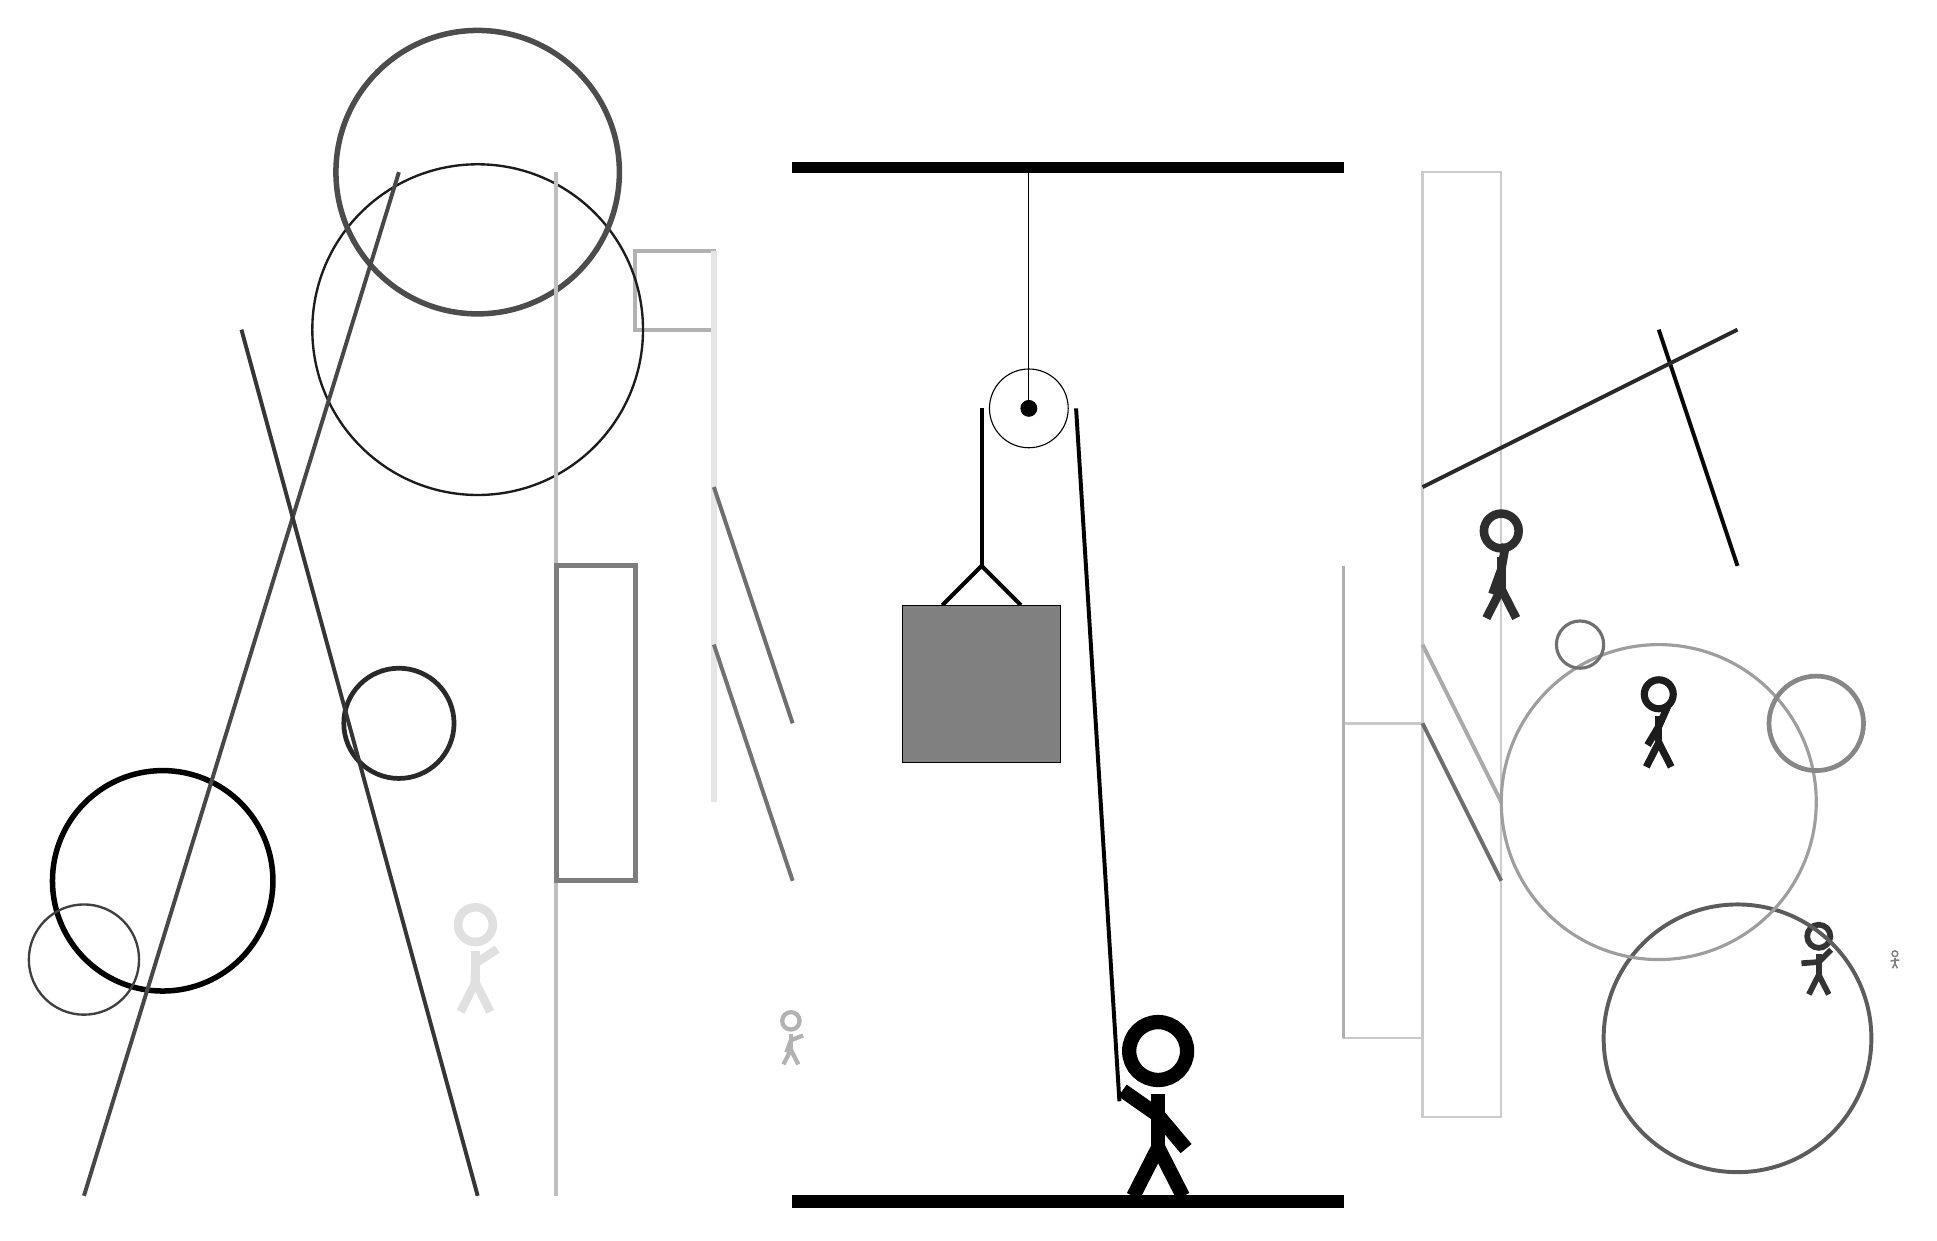
\begin{tikzpicture}
		%%%%% START %%%%%
		
		\draw[fill=black] (-2, 10) rectangle (5, 10.125);
		
		\draw (1, 7) circle (0.5);
		\draw[fill=black] (1, 7) circle (0.1);
		\draw (1, 10) -- (1, 7);
		
		\draw[line width=0.5mm] (-0.1, 4.5) -- (0.4, 5.0) -- (0.9, 4.5);
		\draw[fill=black!50] (-0.6, 4.5) rectangle (1.4, 2.5);
		
		\draw[line width=0.5mm] (0.4, 7) -- (0.4, 5.0);
		\centerarc[line width=0.5mm](1, 7)(0:180:0.6);
		\draw[line width=0.5mm](1.6, 7) -- (2.15, -1.8);
		
		\node at (2.6, -1.9) {\Strichmaxerl[10][-35][-50]};
		
		\draw[line width=0.5mm, color=black!30] (-3, 9) rectangle (-4, 8);
		
		\draw[line width=0.3mm, color=black!20] (6, 10) rectangle (7, -2);
		\draw [line width=0.3mm, color=black!89](-6, 8) circle (2.1);
		\draw [line width=0.6mm, color=black!84](-7, 3) circle (0.7);
		\draw [line width=0.7mm, color=black!70](-6, 10) circle (1.8);
		
		\draw[line width=0.5mm, color=black!21](6, 1) -- (6, 1);
		\draw [line width=0.7mm, color=black!100](-10, 1) circle (1.4);
		\draw [line width=0.3mm, color=black!75](-11, 0) circle (0.7);
		\node[line width=0.5mm, color=black!80] at (11, 0) {\Strichmaxerl[4][4][45]};
		
		\node[line width=0.6mm, color=black!89] at (9, 3) {\Strichmaxerl[5][59][66]};
		\draw[line width=0.5mm, color=black!33](6, 4) -- (7, 2);
		\draw[line width=0.5mm, color=black!97](10, 5) -- (9, 8);
		\node[line width=0.2mm, color=black!12] at (-6, 0) {\Strichmaxerl[6][88][33]};
		\draw [line width=0.5mm, color=black!64](10, -1) circle (1.7);
		\draw [line width=0.4mm, color=black!38](9, 2) circle (2.0);
		\draw[line width=0.5mm, color=black!84](10, 8) -- (6, 6);
		
		\draw[line width=0.7mm, color=black!10] (-3, 9) rectangle (-3, 2);
		\draw[line width=0.3mm, color=black!21] (6, 3) rectangle (5, -1);
		\draw [line width=0.4mm, color=black!56](8, 4) circle (0.3);
		\node[line width=0.6mm, color=black!82] at (7, 5) {\Strichmaxerl[6][70][80]};
		\draw[line width=0.5mm, color=black!25](-5, -3) -- (-5, 10);
		
		\draw [line width=0.6mm, color=black!47](11, 3) circle (0.6);
		\node[line width=0.6mm, color=black!51] at (12, 0) {\Strichmaxerl[1][12][2]};
		\draw[line width=0.6mm, color=black!51] (-4, 1) rectangle (-5, 5);
		\draw[line width=0.4mm, color=black!31] (5, 5) rectangle (5, -1);
		\draw[line width=0.5mm, color=black!72](-7, 10) -- (-11, -3);
		\draw[line width=0.5mm, color=black!57](-2, 3) -- (-3, 6);
		\draw[line width=0.5mm, color=black!79](-6, -3) -- (-9, 8);
		\draw[line width=0.5mm, color=black!57](7, 1) -- (6, 3);
		
		\draw[line width=0.5mm, color=black!55](-2, 1) -- (-3, 4);
		\node[line width=0.2mm, color=black!30] at (-2, -1) {\Strichmaxerl[3][70][21]};
		
		
		\draw[fill=black] (-2, -3) rectangle (5, -3.15);
		
		%%%%% END %%%%%
	\end{tikzpicture}
\end{document}